\section{The chain rule}
\begin{figure}
  \centering
  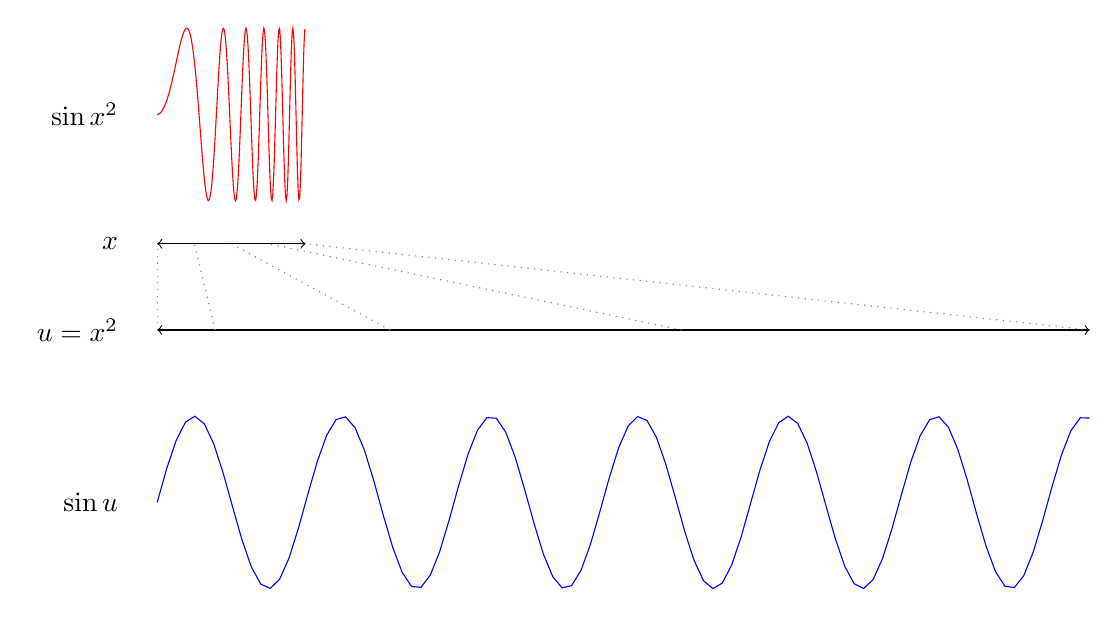
\begin{tikzpicture}
    \begin{axis}[
        axis lines = none,
        scale = 1.5,
        xmin = -7,
        x = 0.2cm
      ]
      \addplot[color = red, domain = 0:2*pi, samples = 200] {sin(deg(x^2)) + 4.5};
      \addplot[color = blue, domain = 0:4*pi^2, samples = 100] {sin(deg(x))};
      \draw[<->] (0, 2) -- (4*pi^2, 2);
      \draw[<->] (0, 3) -- (2*pi, 3);
      \draw (-1.25,2) node[left] {$ u = x^2 $};
      \draw (-1.25,3) node[left] {$ x $};
      \draw (-1.25,0) node[left] {$ \sin u $};
      \draw (-1.25,4.5) node[left] {$ \sin x^2 $};

      \draw[color = gray, style=dotted] (0, 2)      -- (0,3);
      \draw[color = gray, style=dotted] (2.46, 2)   -- (1.57,3);
      \draw[color = gray, style=dotted] (9.86, 2)   -- (3.14,3);
      \draw[color = gray, style=dotted] (22.21, 2)  -- (4.71,3);
      \draw[color = gray, style=dotted] (4*pi^2, 2) -- (2*pi,3);
    \end{axis}
  \end{tikzpicture}
  \caption{A graphic showing how the change of variables $ u \leftrightarrow x^2 $ stretches the graph of $ \sin $.}
\end{figure}

Consider the function $ x \mapsto \sin (x^2) $. This function is made up of two
functions, applied one after the other:
\begin{displaymath}
  x \xmapsto{f} x^2 \xmapsto{g} \sin(x^2).
\end{displaymath}
We often notate this function composition as $ g \circ f $ (note that we
evaluate from the right, so $ (g \circ f)(x) = g(f(x)) $).

Obviously the derivative of $ \sin(x^2) $ is not just $ \cos(2x) $, since the former
has a horizontal tangent line at $ x = \sqrt{\dfrac{\pi}{2}} $ but $ \cos(\sqrt{2\pi}) \neq 0 $. This
shows us that, in general, the derivative of a function composition is not simply the composition
of the derivatives.

In fact, it turns out that the derivative of $ f \circ g $ is $ g' \times (f' \circ g) $; in other words,
\begin{displaymath}
  \od{}{x} f(g(x)) = g'(x) f'(g(x)).
\end{displaymath}
This is known as the \emph{chain rule}, since we are ``chaining'' together functions.

Let us convince ourselves that this rule is plausible. We can interpret the derivative $ \od{g}{x} $ as the rate of change
of $ g $ with respect to $ x $, and the derivative $ \od{f}{g} $ as the derivative of $ f $ with respect to small changes in
the output of $ g $; it is intuitive that if $ g $ changes twice as fast as $ x $ at some point, and $ f $ changes five
times as fast as $ g $, then $ f $ changes $ 2 \times 5 = 10 $ times as fast as $ x $.

The proof goes something like this: consider $ f(g(x + h)) - f(g(x)) $ for small $ h $. We want to write this as $ m h $, where $ m $
is only dependent on $ x $. Now, since $ h $ is small, $ g(x + h) \approx g(x) + g'(x)h $. Thus $ f(g(x + h)) - f(g(x)) \approx f(g(x) + g'(x)h) - f(g(x)) $.
But if $ h $ is small enough, then $ u = g'(x) h $ is small too; so, if $ y = g(x) $, then
\begin{multline*}
  f(g(x + h)) - f(g(x)) \approx f(g(x) + g'(x)h) - f(g(x))\\
    = f(y + u) - f(y) \approx f'(y)u = f'(g(x)) f'(x)h.
\end{multline*}
Thus $ (f \circ g)(x + h) - (f \circ g)(x) \approx f'(g(x)) f'(x) h $, and so $ (f \circ g)'(x) = f'(g(x)) f'(x) $.

\begin{exs}\leavevmode
  \begin{enumerate}
    \item The correct derivative of $ \sin(x^2) $ is $ 2x \cos(x^2) $.
    \item If $ f(r) = \sqrt{r^2 - 3} $, then $ f'(r) = 2r \frac{1}{2} \left(r^2 - 3\right)^{-1/2} = \dfrac{r}{\sqrt{r^2 - 3}} $.
    \item If $ g(x) = \sin((\sin^7 x^7 + 1)^7) $, then we compute:
          \begin{align*}
            g(x)  &= \sin \left( \left[ \left( \sin x^7 \right)^7 + 1 \right]^7 \right)\\
            g'(x) &= 7x^6 \cdot \cos x^7 \cdot 7\left(\sin x^7\right)^6 \cdot 7\left[\left(\sin x^7\right)^7 + 1\right]
                          \cdot \cos \left( \left[ \left( \sin x^7 \right)^7 + 1 \right]^7 \right)
          \end{align*}
  \end{enumerate}
\end{exs}

We can use the chain rule to relate rates of change together --- for example, the area of a circle is given by $ A = \pi r^2 $
and so the rate of change of area with respect to radius $ \od{A}{r} = 2\pi r $; but if $ r $ varies with respect to time then
we can find the rate of change of the area with respect to time using the chain rule.

A useful mnemonic is (if $ x $ is a function of $ y $ which is itself a function of $ z $)
\begin{equation}
  \od{x}{y} \cdot \od{y}{z} = \od{x}{z}. \tag{chain rule}
\end{equation}
We can also apply the inverse function rule for differentiation, which tells us that
\begin{equation}
  \od{x}{y} = \frac{1}{\od{y}{x}}. \tag{inverse function rule}
\end{equation}
The inverse rule is easy to prove: if $ f $ is a function, we have that $ f(f^{-1}(y)) = y $. Taking the derivative of
both sides, $ f'(f^{-1}(y)) \cdot (f^{-1})'(y) = 1 $ and therefore $ (f^{-1})'(y) = \dfrac{1}{f'(f^{-1}(y))} $.

These two operations allow us to rearrange equations as if $ \od{y}{x} $ were a fraction. There isn't much of a problem
if you do think of it in this way, as long as you're careful.

\begin{ex}[Inverse function rule]
  Let us find $ \od{}{x} \tan^{-1} x $. If $ y = \tan^{-1} x $, then $ x = \tan y $; the inverse
  function rule tells us that $ \od{y}{x} = \frac{1}{\od{x}{y}} = \frac{1}{\sec^2 y} = \cos^2 y $.
  Substituting for $ y $, $ \od{y}{x} = (\cos \tan^{-1} x)^2 = \frac{1}{x^2 + 1} $.\footnote{We proved
  that $ \cos \tan^{-1} x = \frac{1}{\sqrt{x^2 + 1}} $ in the trigonometry notes.}
\end{ex}

\begin{ex}
  A ladder \SI{5}{\metre} long rests against a vertical wall. If the bottom of the ladder slides away
  from the wall at a rate of \SI{1}{\metre\per\second}, how fast is the top of the ladder sliding down the
  wall when the bottom of the ladder is \SI{3}{\metre} from the wall?

  \textit{Solution.} Let $ x $ be the distance of the bottom of the ladder from the wall, and let $ y $
  be the height of the top of the ladder up the wall. We have $ \od{x}{t} = 1 $ and $ x = 3 $; we also
  know that $ y = \sqrt{25 - x^2} $, so:
  \begin{align*}
    \dod{y}{t} &= \dod{y}{x} \cdot \dod{x}{t} = -\frac{x}{\sqrt{25 - x^2}} \cdot 1\\
    \eval{\dod{y}{t}}_{x = 3} &= -\frac{3}{\sqrt{25 - 9}} = -\frac{3}{4}.
  \end{align*}
  Hence the ladder is sliding down the wall at a rate of \SI{-0.75}{\metre\per\second}.
\end{ex}

\begin{ex}
  The radius of a sphere is increasing at a rate of $ \od{r}{t} = -\ln(t - 1) $ metres per second. At what rate will the surface area of
  the sphere be growing at $ t = 2 $?

  \textit{Solution.} We have $ \mathrm{SA} = 4\pi r^2 $, so $ \od{\mathrm{SA}}{r} = 8\pi r $ and
    \begin{displaymath}
      \od{\mathrm{SA}}{t} = \od{\mathrm{SA}}{r} \od{r}{t} = -\ln(t - 1) \times 8\pi r = 0.
    \end{displaymath}

    The surface area of the sphere will be momentarily constant at $ t = 2 $.
\end{ex}

\subsection{Exercises and Problems}
\begin{enumerate}
  \item Identify the inner and outer functions, but don't try to differentiate.
    \begin{enumerate}
      \item $ \sqrt{\sin x} $
      \item $ \sin \cos \tan x $
      \item $ (2x + 3)^{17} $
      \item $ 97(x + 2)^2 $
      \item $ \ln \sin x $
      \item $ \frac{1}{\sqrt{23x - x^2}} $
    \end{enumerate}
  \item Differentiate with respect to $ t $:
    \begin{multicols}{2}
    \begin{enumerate}
      \item $ (2t + 3)^{3000} $
      \item $ \sin \ln t $
      \item $ \sqrt{t^3 + 10t^2 + 3} $
      \item $ \csc e^t $
      \item $ \sin^3 t + 14\ln (3t) $
      \item $ \sin \sin \sin t $
      \item $ \cot (t + \sec t) $
      \item $ \sin^2 ((t + \sin t)^2) $
      \item $ \ln \sqrt{t + 9} $
      \item $ \sqrt{t} + \frac{1}{\sqrt[3]{t^4}} $
      \item $ e^{\sec (t^2)} $
      \item $ \sin \sqrt{t + \tan t} $
    \end{enumerate}
    \end{multicols}
  \item The derivative of a function is $ 2 \cos 2x $. What could the original function be?
  \item Differentiate $ y = \sin^2 x + \cos^2 x $, and hence prove that $ \sin^2 x + \cos^2 x = 1 $.
  \item Suppose that the displacement of a particle on a vibrating spring is given by $ x(t) =  5 + \frac{1}{8} \sin(5\pi t) $,
        where $ x $ is measured in centimetres and $ t $ in seconds.
    \begin{enumerate}
      \item Find the velocity of the particle at time $ t $.
      \item At which times is the particle momentarily stationary?
    \end{enumerate}
  \item Find a linear approximation $ \tilde f $ around 0 for $ f(x) = \sqrt[4]{1 + 2x} $; then calculate $ \delta $ such that
        for all $ x $ satisfying $ -\delta < h < \delta $, $ -0.1 < \tilde f(x) - f(x) < 0.1 $.
  \item The volume of a spherical balloon at a time $ t $ is given by $ V(t) = \frac{4}{3} \pi r^2 $, and its radius, changing
        over time, is given by $ r(t) $. Find $ \od{V}{t} $ in terms of $ \od{r}{t} $.
  \item If $ F(x) = f(3f(4f(x))) $, where $ f(0) = 0 $ and $ f'(0) = 2 $, find $ F'(0) $.
  \item Suppose $ f(x) = g(x + g(a)) $ for some differentiable function $ g $ and constant $ a $. Find $ f'(x) $.
  \item The depth of water at the end of a jetty in a harbour varies with time due to the tides. The depth
        of the water is given by the formula
        \begin{displaymath}
          W = 4.5 - 1.2 \cos \frac{\pi t}{6}
        \end{displaymath}
        where $ W $ is the water depth in metres, and $ t $ is the time in hours after midnight.
    \begin{enumerate}
      \item What is the rate of change of water depth 5 hours after midnight?
      \item When is the first time after $ t = 0 $ that the tide changes direction?
      \item At that time, is the water changing from rising to falling or from falling to rising?
    \end{enumerate}
  \item In physics, the rate of change of momentum of an object is proportional to the force needed to effect
        that change: if $ p $ is the momentum of the object as a function of time, $ F = \od{p}{t} $. The momentum
        of a particular object, oscillating back and forth along a line, is given by $ p = mA\sin(\omega t + \phi)\thinspace\si{\kilo\gram\metre\per\second} $
        (where $ m $, $ A $, $ \omega $, and $ \phi $ are various constants). What is the force acting on the object at $ t = 10 $?
  \item Find the 73rd derivative of $ \sin 6x $.
  \item Each side of a square is increasing at a rate of \SI{6}{\centi\metre\per\second}. At what rate is the
        area of the square increasing when the area of the square is \SI{16}{\centi\metre\squared}?
  \item Gas is being forced into a spherical balloon at a rate of \SI{400}{\centi\metre\cubed\per\minute}. How fast
        is the radius of the balloon increasing when the radius is \SI{5}{\centi\metre}?
  \item If a snowball melts so that its surface area decreases at a rate of \SI{1}{\centi\metre\squared\per\minute}.
        find the rate at which the diameter decreases when the diameter is \SI{10}{\centi\metre}.
  \item If $ x^2 + y^2 + z^2 = 9 $, $ \od{x}{t} = 5 $, and $ \od{y}{t} = 4 $, find $ \od{z}{t} $ when $ (x,y,z) = (2,2,1) $.
  \item A particle moves along the curve $ y = 2\sin(\pi x/2) $. As the particle moves through the point $ (1/3, 1) $,
        its $ x$-ordinate increases at a rate of $ \sqrt{10} $ \si{\centi\metre\per\second}. How fast is the distance
        from the particle to the origin changing at this instant?
  \item Gravel is dumped from a conveyor belt at a rate of \SI{3}{\metre\cubed\per\minute}, and forms a pile in the shape
        of a cone with equal height and base diameter. How fast is the height of the cone increasing when the pile is \SI{3}{\metre}
        tall?
  \item The top of a ladder slides down a vertical wall at a rate of \SI{0.15}{\metre\per\second}. A the moment when the bottom
        of the ladder is \SI{3}{\metre} from the bottom of the wall, it slides away from the wall at a rate of \SI{0.2}{\metre\per\second}.
        Find the length of the ladder.
  \item Two sides of a triangle have lengths \SI{2}{\metre} and \SI{3}{\metre}. The angle between these sides is increasing
        at a rate of \SI{4}{\degree\per\second}. How fast is the length of the third side changing when it is of length \SI{4}{\metre}?
  \item A particle is moving along a hyperbola $ xy = 8 $. As it reaches the point $ (4, 2) $, the $ y$-ordinate is decreasing
        at a rate of 3 units per second. How fast is the $ x$-ordinate of the particle changing at that instant?
  \item The minute hand on a watch is \SI{8}{\milli\metre} long and the hour hand is \SI{4}{\milli\metre} long. How fast is the
        distance between the tips of the hands changing at 1 o'clock?
  \item If $ f(\theta) = \sin^{-1} (\theta) $, compute $ \od{}{\theta} f(\theta) $ and $ \od{}{x} f(x^4) $.
  \item Recall that the \emph{absolute value} of $ x $, denoted $ \abs{x} $, is the value obtained by `throwing away the sign' of $ x $.
    \begin{enumerate}
      \item Prove that
            \begin{displaymath}
              \od{}{x} \abs{x} = \frac{x}{\abs{x}}.
            \end{displaymath}
            [\textit{Hint: Write $ \abs{x} = \sqrt{x^2} $.}]
      \item If $ f(x) = \abs{\sin x} $, find $ f'(x) $ and sketch the graphs of both $ f $ and $ f' $.
    \end{enumerate}
  \item Note that on the formula sheet, the anti-derivative of $ 1/x $ is given as $ \ln \abs{x} $, not just $ \ln x $.
    \begin{enumerate}
      \item Compute $ \od{}{x} \ln \abs{x} $ if $ x < 0 $, and hence justify formally why $ \od{}{x} \ln \abs{x} = 1/x $.
      \item Draw $ y = \ln \abs{x} $ and $ y = 1/x $ on the same pair of axes, and hence justify intuitively why $ \od{}{x} \ln \abs{x} = 1/x $.
    \end{enumerate}
  \item Soon, we will be studying the product rule for derivatives. It is possible, though not
        particularly usual, to prove it using simply the basic derivatives from the last section and the chain
        rule; in this exercise, you will do just that.

        Suppose that $ f $ and $ g $ are functions, and consider the function $ F $ defined by $ F(x) = \left(f(x) + g(x)\right)^2 $.
    \begin{enumerate}
      \item Calculate $ F'(x) $ using the chain rule.
      \item Calculate $ F'(x) $ by multiplying out the square and differentiating the polynomial that results. (In particular, note
            that $ \od{}{x} 2(fg)(x) = 2 (fg)'(x) $).
      \item Compare parts (a) and (b).
    \end{enumerate}
\end{enumerate}

\subsection{References}
For an approach to the chain rule similar to the one taken here, see chapter IX of Thompson. See also sections 2.5 and 2.8 of Stewart.

\subsection{Homework}
\paragraph{Reading}
Historically, when Leibniz conceived of the notation, $ \od{y}{x} $ was supposed to be a quotient: it was the quotient of the ``infinitesimal change in $y$ produced by the change in $x$'' divided by the ``infinitesimal change in $x$''.

However, the formulation of calculus with infinitesimals in the usual setting of the real numbers leads to a lot of problems. For one thing, infinitesimals can't exist in the usual setting of real numbers! This is because the real numbers satisfy an important property, called the Archimedean property: given any positive real number $ \varepsilon > 0 $, no matter how small, and given any positive real number $ N > 0 $, no matter how big, there exists a natural number $n$ such that $n \varepsilon > N$. An ``infinitesimal'' $ \xi $ is supposed to be so small that no matter how many times you add it to itself, it never gets to 1, contradicting the Archimedean property.

Other problems: Leibniz defined the tangent to the graph of $y=f(x)$ at $x=a$ by saying "Take the point $(a,f(a))$; then add an infinitesimal amount to $a$, $a+\dif{x}$, and take the point $(a+dx,f(a+\dif{x}))$, and draw the line through those two points." But if they are two different points on the graph, then it's not a tangent, and if it's just one point, then you can't define the line because you just have one point. That's just two of the problems with infinitesimals.

So calculus was essentially rewritten from the ground up in the following 200 years to avoid these problems, and you are seeing the results of that rewriting. Because of that rewriting, the derivative is no longer a quotient, now it's a limit:
\begin{displaymath}
  \lim_{h \to 0} \frac{f(x + h) - f(x)}{h}
\end{displaymath}

Because we cannot express this limit-of-a-quotient as a-quotient-of-the-limits (both numerator and denominator go to zero), then the derivative is not a quotient.
However, Leibniz' notation is very suggestive and very useful; even though derivatives are not really quotients, in many ways they behave as if they were quotients. So we have the chain rule:
\begin{displaymath}
  \od{y}{x} = \od{y}{u} \od{y}{x}
\end{displaymath}
which looks very natural if you think of the derivatives as ``fractions''. You have the inverse function theorem, which tells you that
\begin{displaymath}
  \od{x}{y} = 1/\od{y}{x}
\end{displaymath}
which is again almost ``obvious'' if you think of the derivatives as fractions. So, because the notation is so nice and so suggestive, we keep the notation even though the notation no longer represents an actual quotient: it now represents a single limit.  Even though we write $ \od{y}{x} $ as if it were a fraction, and many computations look like we are working with it like a fraction, it isn't really a fraction (it just plays one on television).

There is a way of getting around the logical difficulties with infinitesimals; this is called nonstandard analysis. It's pretty difficult to explain how one sets it up, but you can think of it as creating two classes of real numbers: the ones you are familiar with, that satisfy things like the Archimedean property, the least-upper-bound property, and so on, and then you add another, separate class of real numbers that includes infinitesimals and a bunch of other things. If you do that, then you can, if you are careful, define derivatives exactly like Leibniz, in terms of infinitesimals and actual quotients; if you do that, then all the rules of calculus that make use of $ \od{y}{x} $ as if it were a fraction are justified because, in that setting, it is a fraction. Still, one has to be careful because you have to keep infinitesimals and regular real numbers separate and not let them get confused, or you can run into some serious problems.

\begin{flushright}
  Arturo Magidin (\url{https://math.stackexchange.com/users/742/arturo-magidin}), Is $\od{y}{x}$ not a ratio? (adapted), URL (version: 2017-09-15): \url{https://math.stackexchange.com/q/21209}
\end{flushright}


\paragraph{Problems}
\begin{enumerate}
  \item If $ y = \sqrt{\cot x} - \sqrt{\cot a} $ (where $ a $ is constant), find $ \od{y}{x} $.
  \item
    \begin{enumerate}
      \item Show that if $ y = f(g(h(x))) $ then $ \od{y}{x} = h'(x) \cdot g'(h(x)) \cdot f'(g(h(x))) $.
      \item Calculate the derivative of $ y = \sin \cos \sin \cos \sin x^5 $.
    \end{enumerate}
  \item We will prove the double angle formula for cosine from the double angle formula for sine.
            Suppose $ f(\theta) = \cos 2\theta $, and $ g(\theta) =  1 - 2\sin^2 \theta $.
    \begin{enumerate}
      \item Show that $ f' = g' $. (You may assume that $ \sin 2\theta = 2\sin \theta \cos \theta $.)
      \item Verify that $ f $ and $ g $ agree at $ \theta = 0 $, and conclude that $ f = g $.
    \end{enumerate}
  \item If $ V $ is the volume of a cube with edge length $ x $ and the cube expands as time passes,
        find $ \od{V}{t} $ in terms of $ \od{x}{t} $.
  \item A water tank has the shape of an inverted circular cone with base radius \SI{2}{\metre}
        and height \SI{4}{\metre}. If water is being pumped into the tank at a rate of \SI{2}{\metre\cubed\per\minute},
        find the rate at which the water level is rising when the water is \SI{3}{\metre} deep.
  \item A boat is pulled into a dock by a rope attached to the bow of the boad and passing through a pulley on
        the dock that is \SI{1}{\metre} higher than the bow of the boat. If the rope is pulled in at a rate
        of \SI{1}{\metre\per\second}, how fast is the boat approaching the dock when it is \SI{8}{\metre} from the dock?
\end{enumerate}
